% Here describe how did you come with your solution.
% In this section you need to describe:

% \begin{itemize}
%     \item What are you supposed to do, and why is it \emph{sound}.
%     \item What did you do, and what \emph{happened}
%     \item Provide a diagram of the software architecture of what you built. Remember there are various types of diagrams (e.g., contextual, structural, etc). Identify what the best diagram is for the purpose of your contribution.
% \end{itemize}

% All in all, this is the meat of the work, please show information about why what you did is important and how will you carry it forward.
% 1-2 pages is reasonable for this.

% arch.tex
% \section{System Architecture and Approach}
Our solution rests on two core components—a malicious test server and custom Scrapy spiders—glued together by a Flask orchestration UI.

\begin{itemize}
  \item \textbf{Malicious Flask Server:} Hosts endpoints for SQLi (`/sqli`), reflected XSS (`/xss_script`), and malware downloads (`/malware`), each intentionally lacking sanitization or content validation.
  \item \textbf{Scrapy Spiders:}
    \begin{itemize}
      \item \emph{SQLi Spider:} Submits FormRequests with tautologies and destructive payloads.
      \item \emph{XSS Spider:} Uses `scrapy-playwright` to render pages and override `window.alert()` via `add_init_script`.
      \item \emph{Malware Spider:} Follows download links and saves binaries without inspection.
    \end{itemize}
  \item \textbf{Flask Orchestration UI:} Provides “Trigger Crawl” buttons, in‐memory logging, and a live `/logs` dashboard (auto‐refresh).
\end{itemize}

\begin{figure*}[!t]
  \centering
  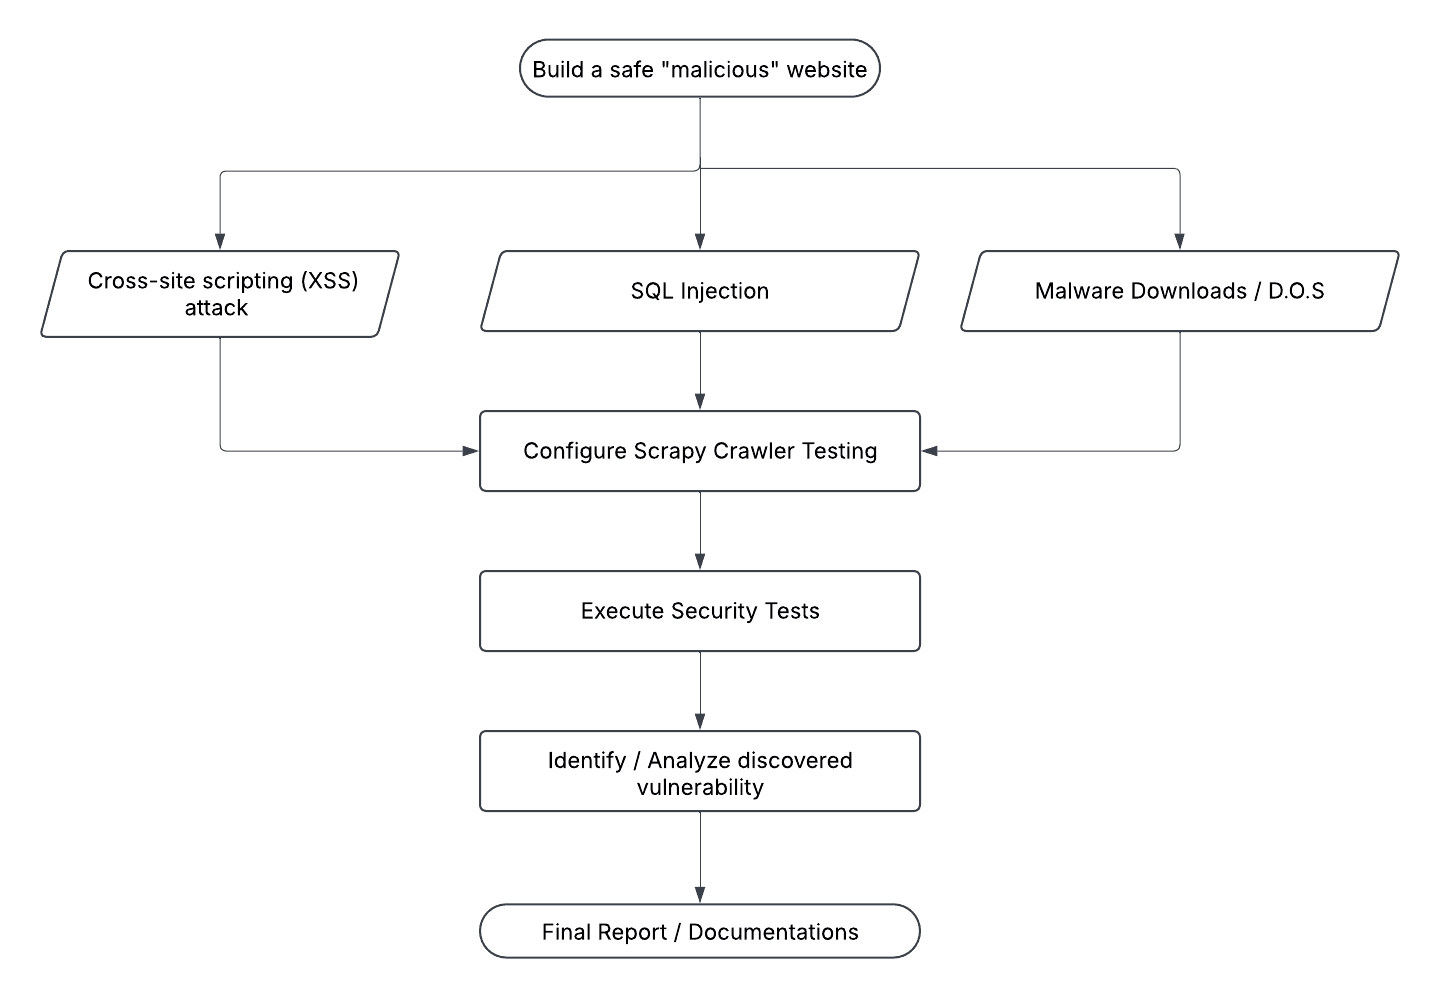
\includegraphics[width=\textwidth]{figures/blockarch.png}
  \caption{System architecture of ScrapyShield.}
  \label{fig:architecture}
\end{figure*}
